\documentclass[t]{beamer}
\usetheme[deutsch]{KIT}
\setbeamercovered{transparent}
\setbeamertemplate{navigation symbols}{}

\KITfoot{YUV.KA - Praxis der Softwareentwicklung WS 11/12}
\usepackage[utf8]{inputenc}
\usepackage{ngerman}
\usenavigationsymbols

\title{YUV.KA}
\subtitle{Abschlusspräsentation Entwurfsphase}
\author{Max Wagner $\cdot$ Patrick Gemander $\cdot$ Sebastian Ullrich $\cdot$ Michael Vollmer \\ Robert Hangu $\cdot$ Daniel Lebert}

\institute[ITEC]{Institut für Technische Informatik}

\TitleImage[trim = -20cm 0 0 0,height=\titleimageht]{../logo.png}

\begin{document}

\begin{frame}
\maketitle
\end{frame}
 
\begin{frame}
\frametitle{MVVM (Model-View-ViewModel)}
\noindent
\begin{minipage}{3.5cm}
    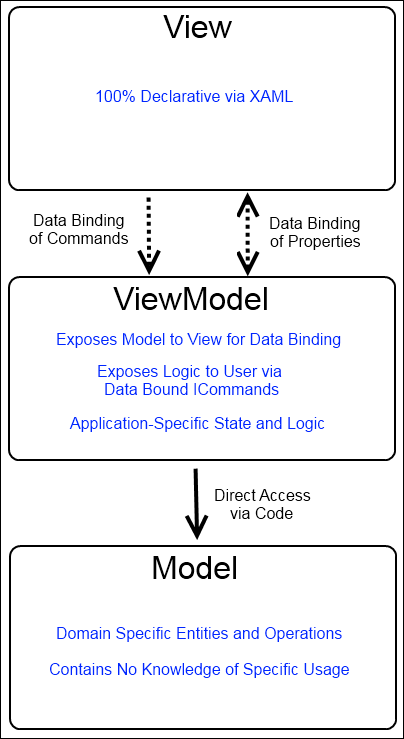
\includegraphics[width=3.5cm]{MVVM_thumb.png}

    \textit{http://reedcopsey.com}
\end{minipage}
\hfill
\begin{minipage}{8cm}
    \begin{itemize}
        \item Eigens für WPF entwickeltes Entwurfsmuster
        \item Erzielt Modularität und Testbarkeit durch vollständige Entkopplung von UI-Elementen und UI-Logik
    \end{itemize}
\end{minipage}
\end{frame}

\begin{frame}
\frametitle{Umsetzung}
\begin{center}
    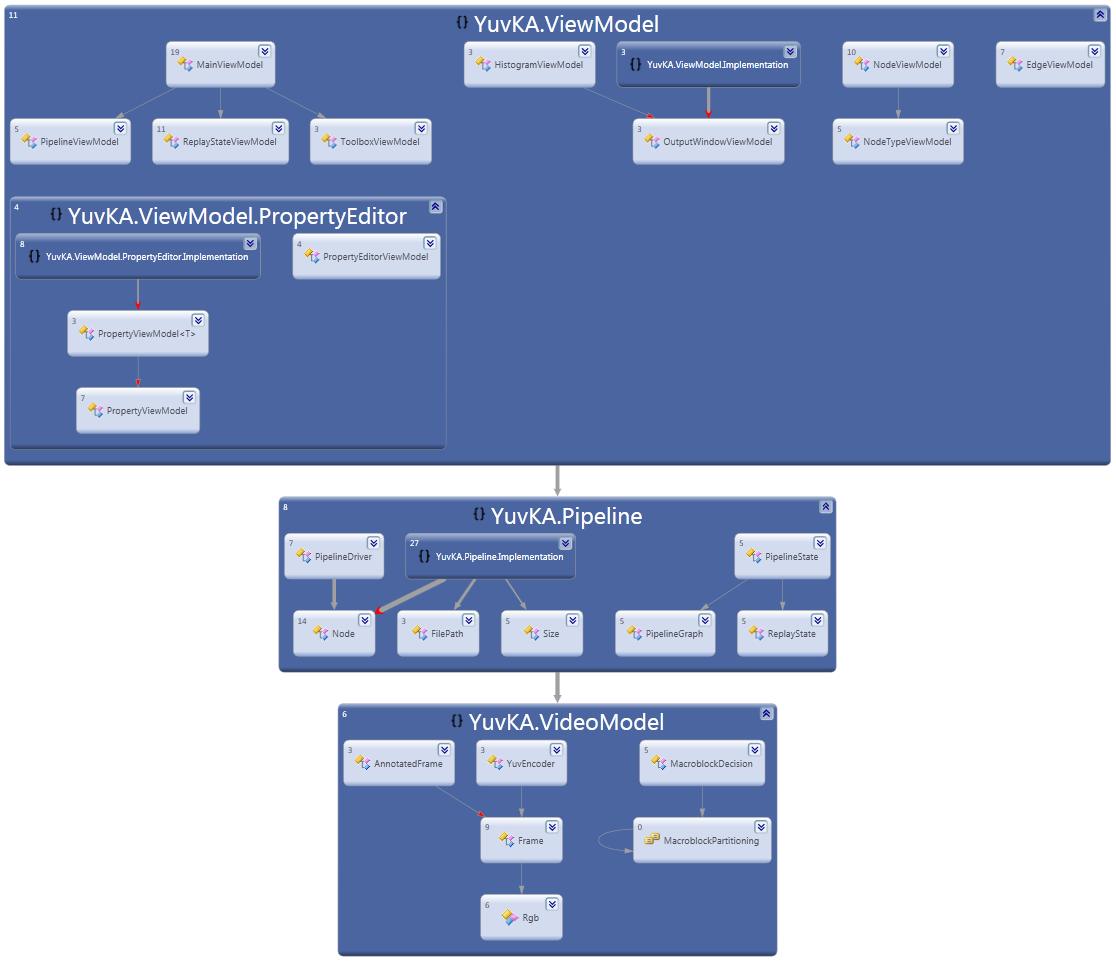
\includegraphics[height=0.9\textheight]{../Diagrams/namespacedependencies.png}
\end{center}
\end{frame}

\begin{frame}
\frametitle{Video Model}
\noindent
\begin{minipage}{5cm}
    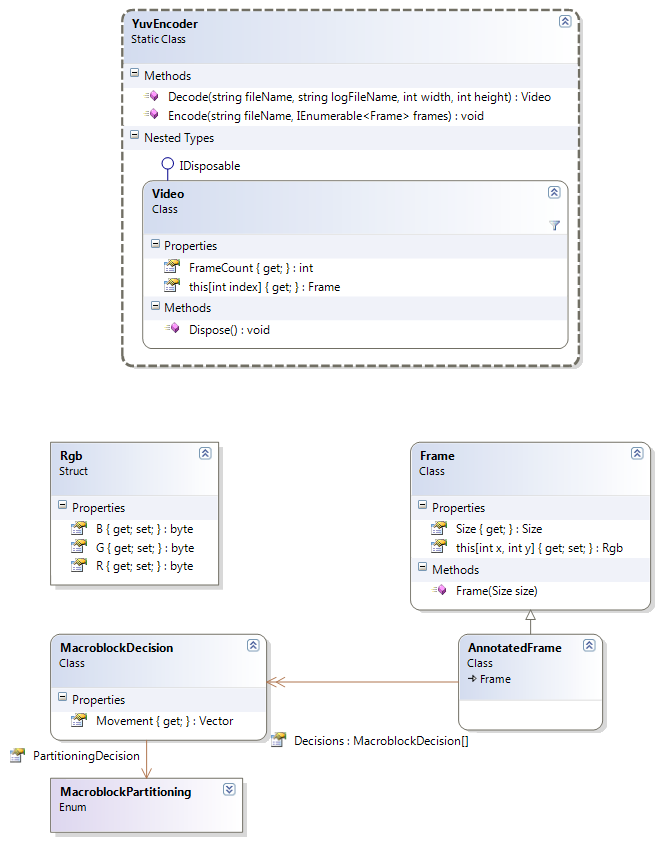
\includegraphics[height=0.9\textheight]{../YuvKA.VideoModel/videomodel.png}
\end{minipage}
\hfill
\begin{minipage}{6cm}
    \begin{itemize}
        \item Speichert YUV-Videos im RGB-Format
        \item Zusätzlich können Metadaten über Encoder-Entscheidungen eingelesen werden
    \end{itemize}
\end{minipage}
\end{frame}

\begin{frame}
\frametitle{Pipeline}
\noindent
\begin{minipage}{5cm}
    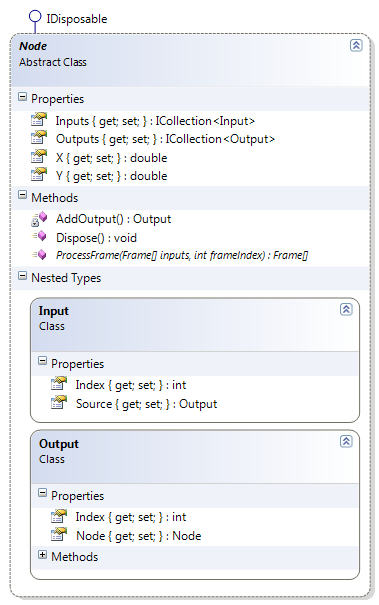
\includegraphics[height=0.9\textheight]{../YuvKA.Pipeline/node.png}
\end{minipage}
\hfill
\begin{minipage}{6cm}
    \begin{itemize}
        \item Gerichteter azyklischer Graph aus Knoten, die Frame-Eingaben in -Ausgaben konvertieren
        \item Driver berechnet den Graph für mehrere Ticks parallel
    \end{itemize}
\end{minipage}
\end{frame}

\begin{frame}
\frametitle{View Model}
\noindent
\begin{minipage}{5cm}
    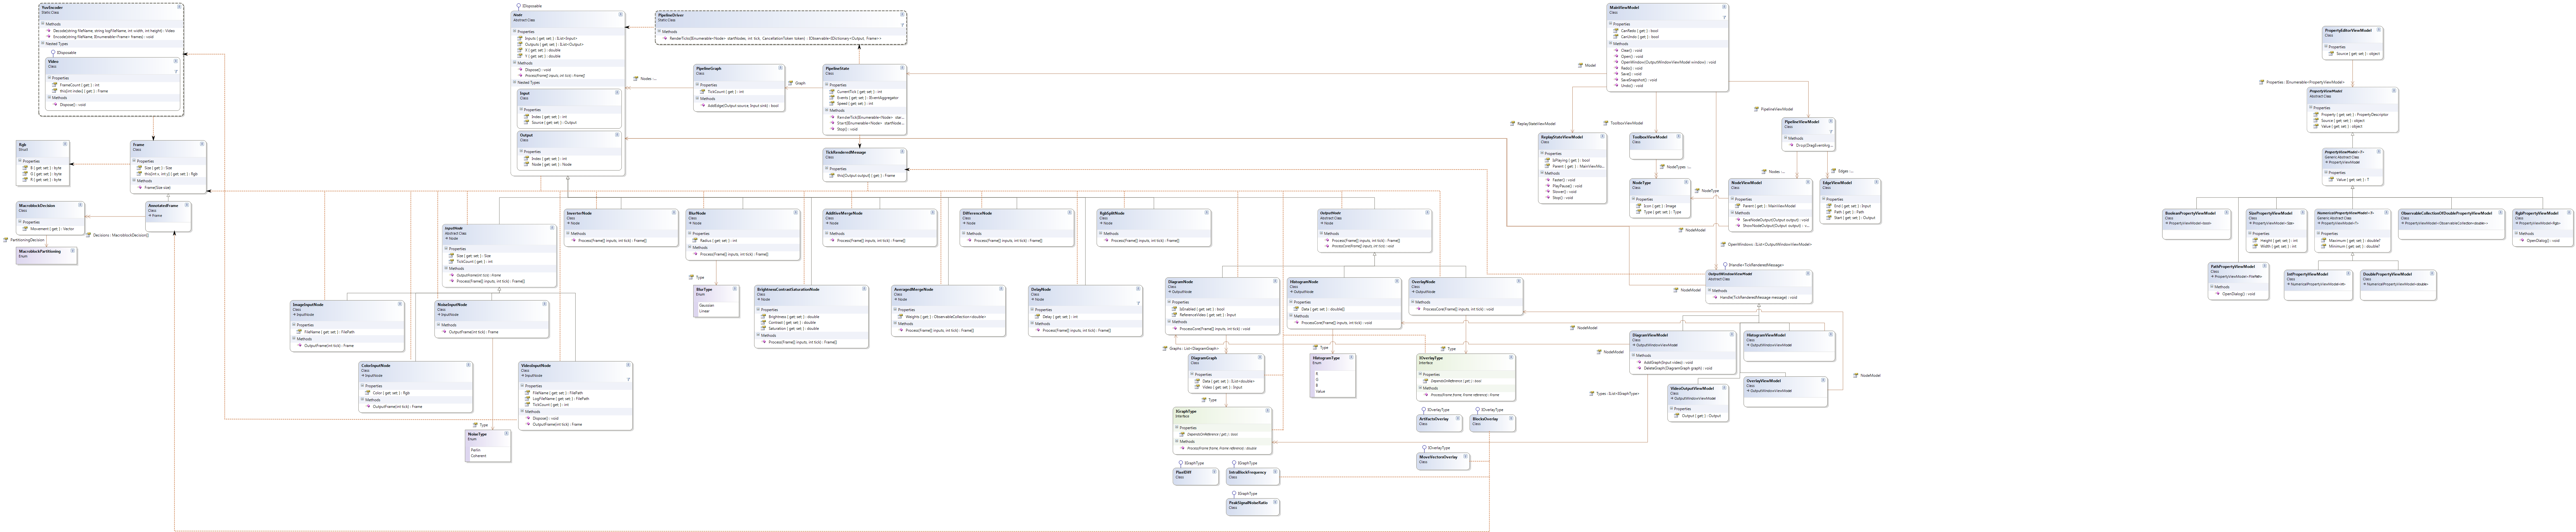
\includegraphics[trim=135cm 5cm 50cm 0,clip,height=\textheight]{../Diagrams/classdiagram.png}
\end{minipage}
\hfill
\begin{minipage}{5.5cm}
    \begin{itemize}
        \item ``Value Converter'' zwischen Model und View
        \item Einzelne UI-Bereiche werden auf eigene View Models abgebildet
    \end{itemize}
\end{minipage}
\end{frame}

\begin{frame}
\frametitle{Property Editor}
\noindent
\begin{minipage}{6cm}
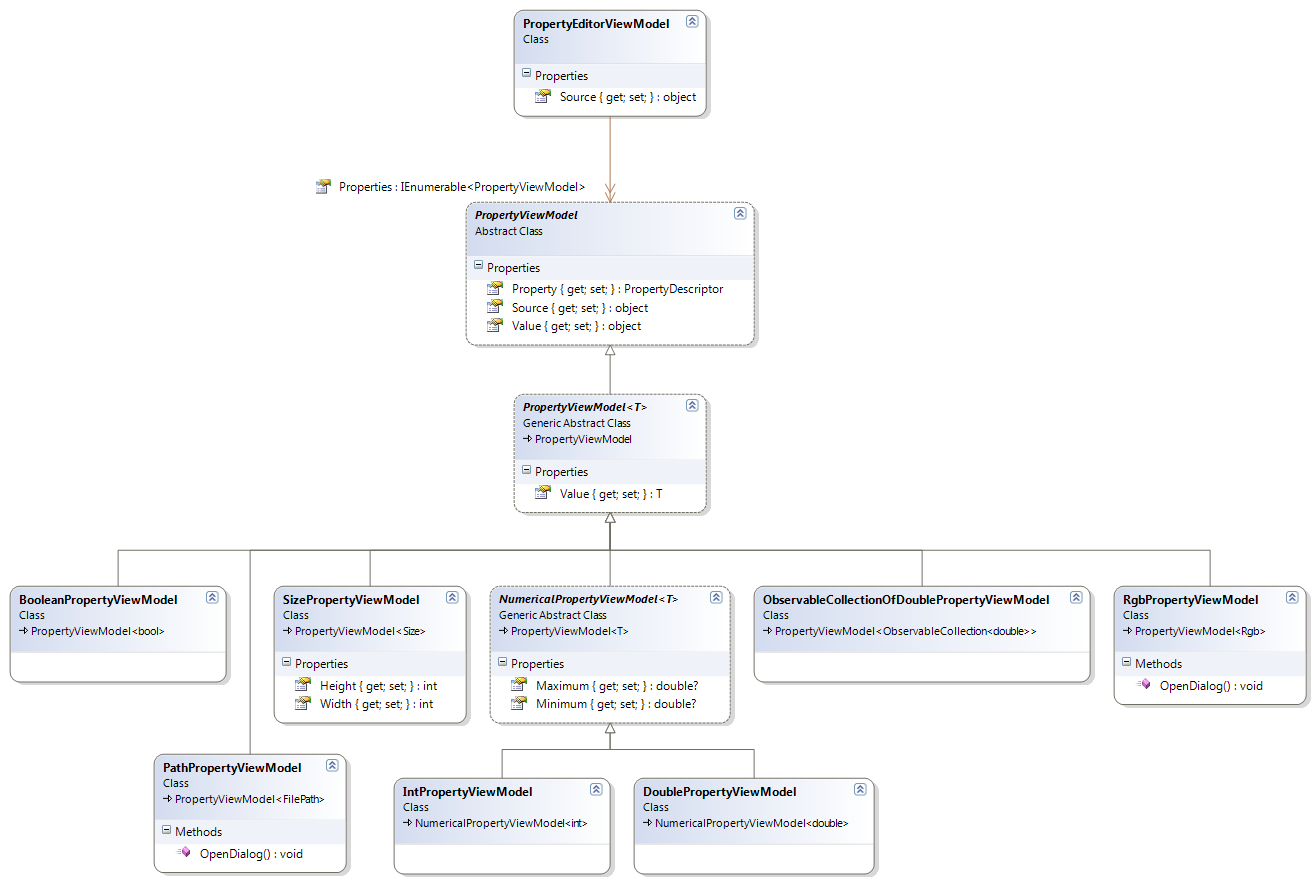
\includegraphics[height=0.9\textheight]{../YuvKA.ViewModel.PropertyEditor/propertyEditor.png}
\end{minipage}
\hfill
\begin{minipage}{5cm}
    \vspace{-2cm} %haxx
    \begin{itemize}
        \item Eigenständige Komponente
        \item Listet Propertywerte eines Objektes auf
        \item Controls werden dynamisch je nach Propertytyp erstellt
    \end{itemize}
\end{minipage}
\end{frame}

\end{document}
